\section{Introduction}

\begin{frame}{Magnetic Levitation System (MLS)}

    Magnetic Levitation System (MLS) is an electromechanical system that enhances magnetic fields to levitate a ferromagnetic object.
    It's known for its non-linear behavior and its instability.

    \begin{figure}[H]
        \centering
        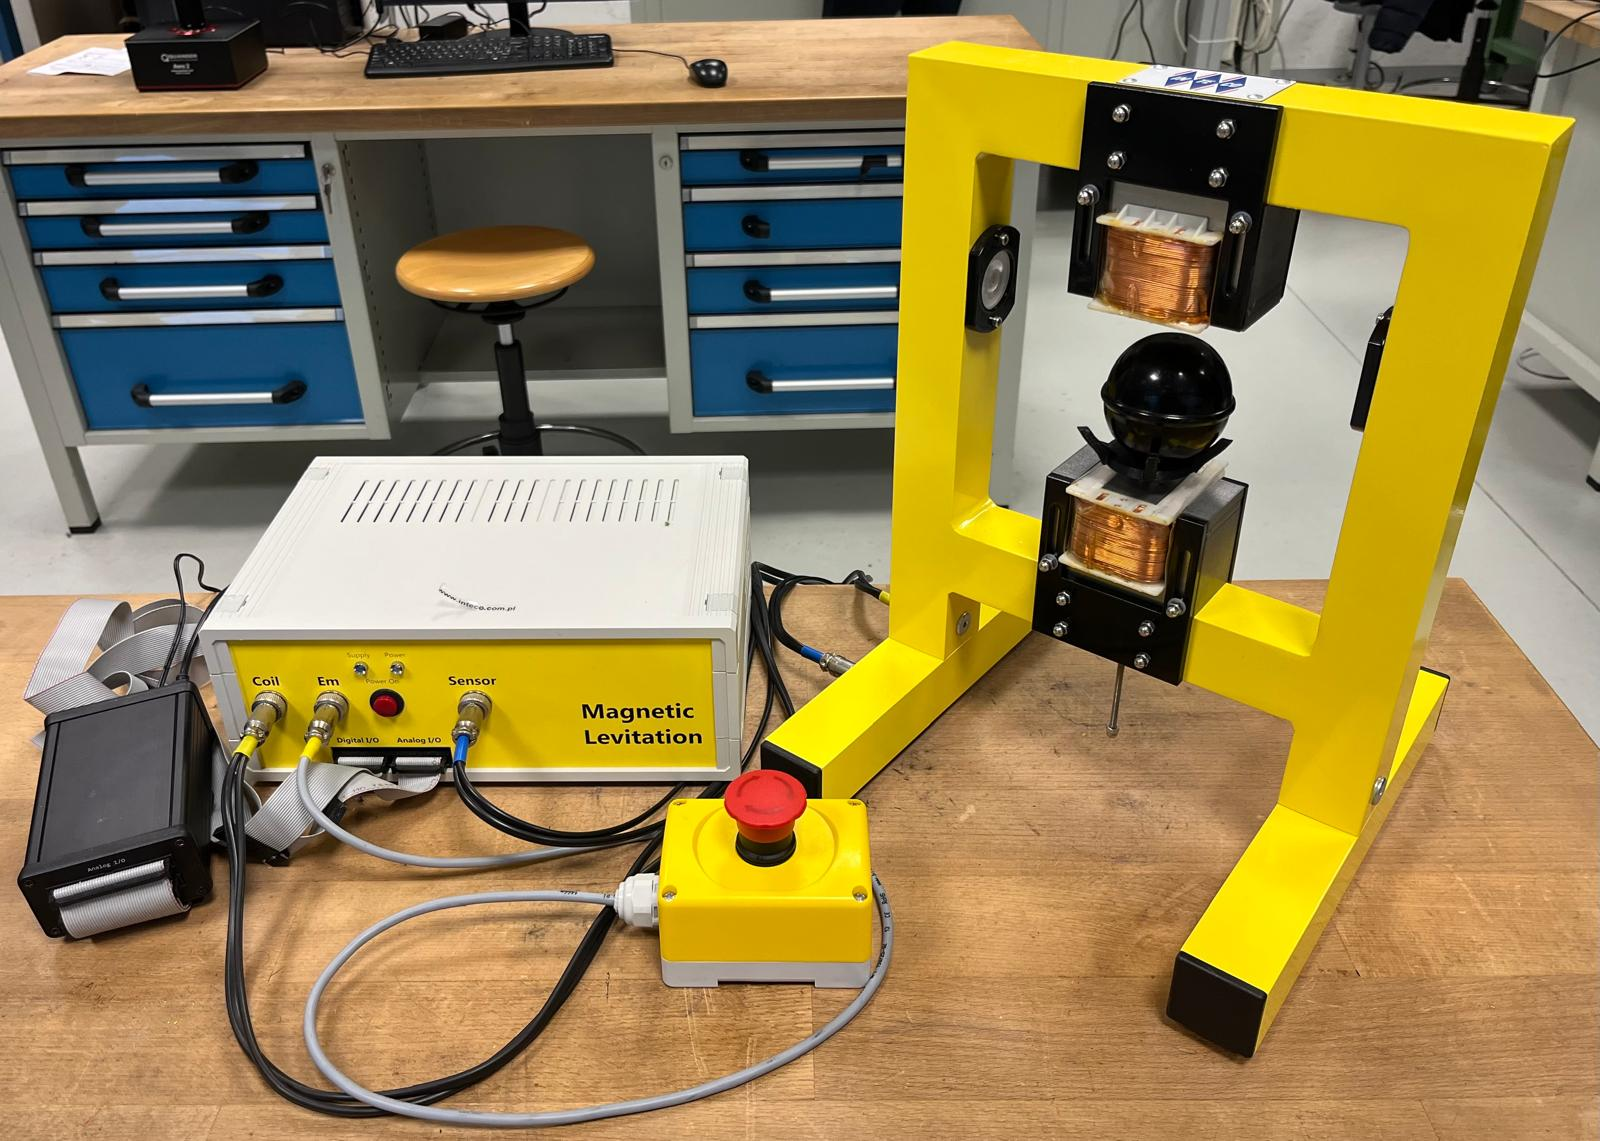
\includegraphics[width=0.5\textwidth]{./img/Maglev_from_the_lab.jpeg}
        \caption{Magnetic Levitation System used in this work.}
    \end{figure}

    The variable magnetic field is generated by two electromagnets driven in voltage, while the position of the ball is measured by an optical infrared sensor.

\end{frame}



\begin{frame}{Project objectives}

    \vspace{9pt}

    \begin{columns}[c, onlytextwidth]

        \begin{column}{0.5\textwidth}

            \begin{figure}[H]
                \centering
                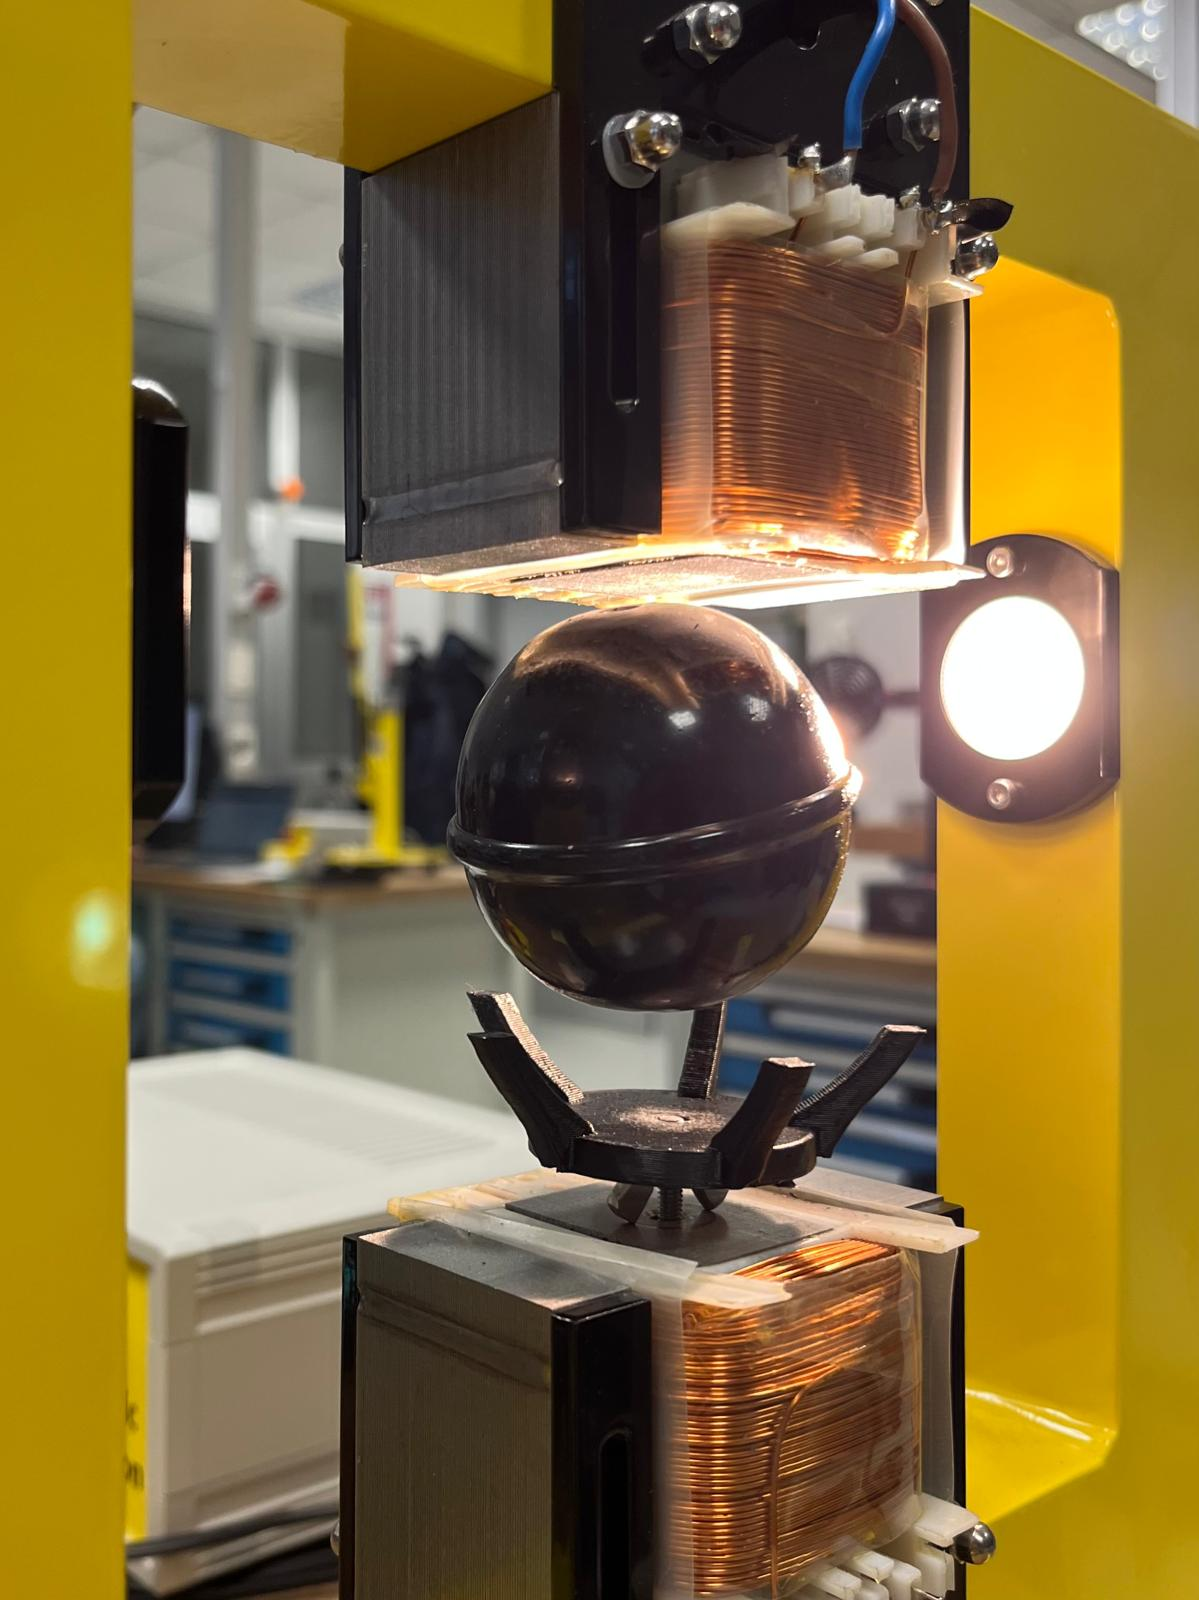
\includegraphics[width=0.8\textwidth]{./img/ball_levitation.jpeg}
                \caption{Sphere levitating}
            \end{figure}

        \end{column}

        \begin{column}{0.5\textwidth}

            \begin{center}
                Project objectives: \\
                \textbf{Make the ball levitate.}
            \end{center}

        \end{column}

    \end{columns}

\end{frame}


